\subsubsection{Testes} % (fold)
\label{ssub:testes}

Quando uma fase ainda se encontra aberta para submissões, o docente pode adicionar testes que permitem ajudar o mesmo no processo de avaliação. Estes testes são executados quando um aluno faz uma submissão.

Na Figura~\ref{fig:tests} pode ser consultada uma imagem demonstrativa da página desenvolvida.

\begin{figure}[H]
  \centering
  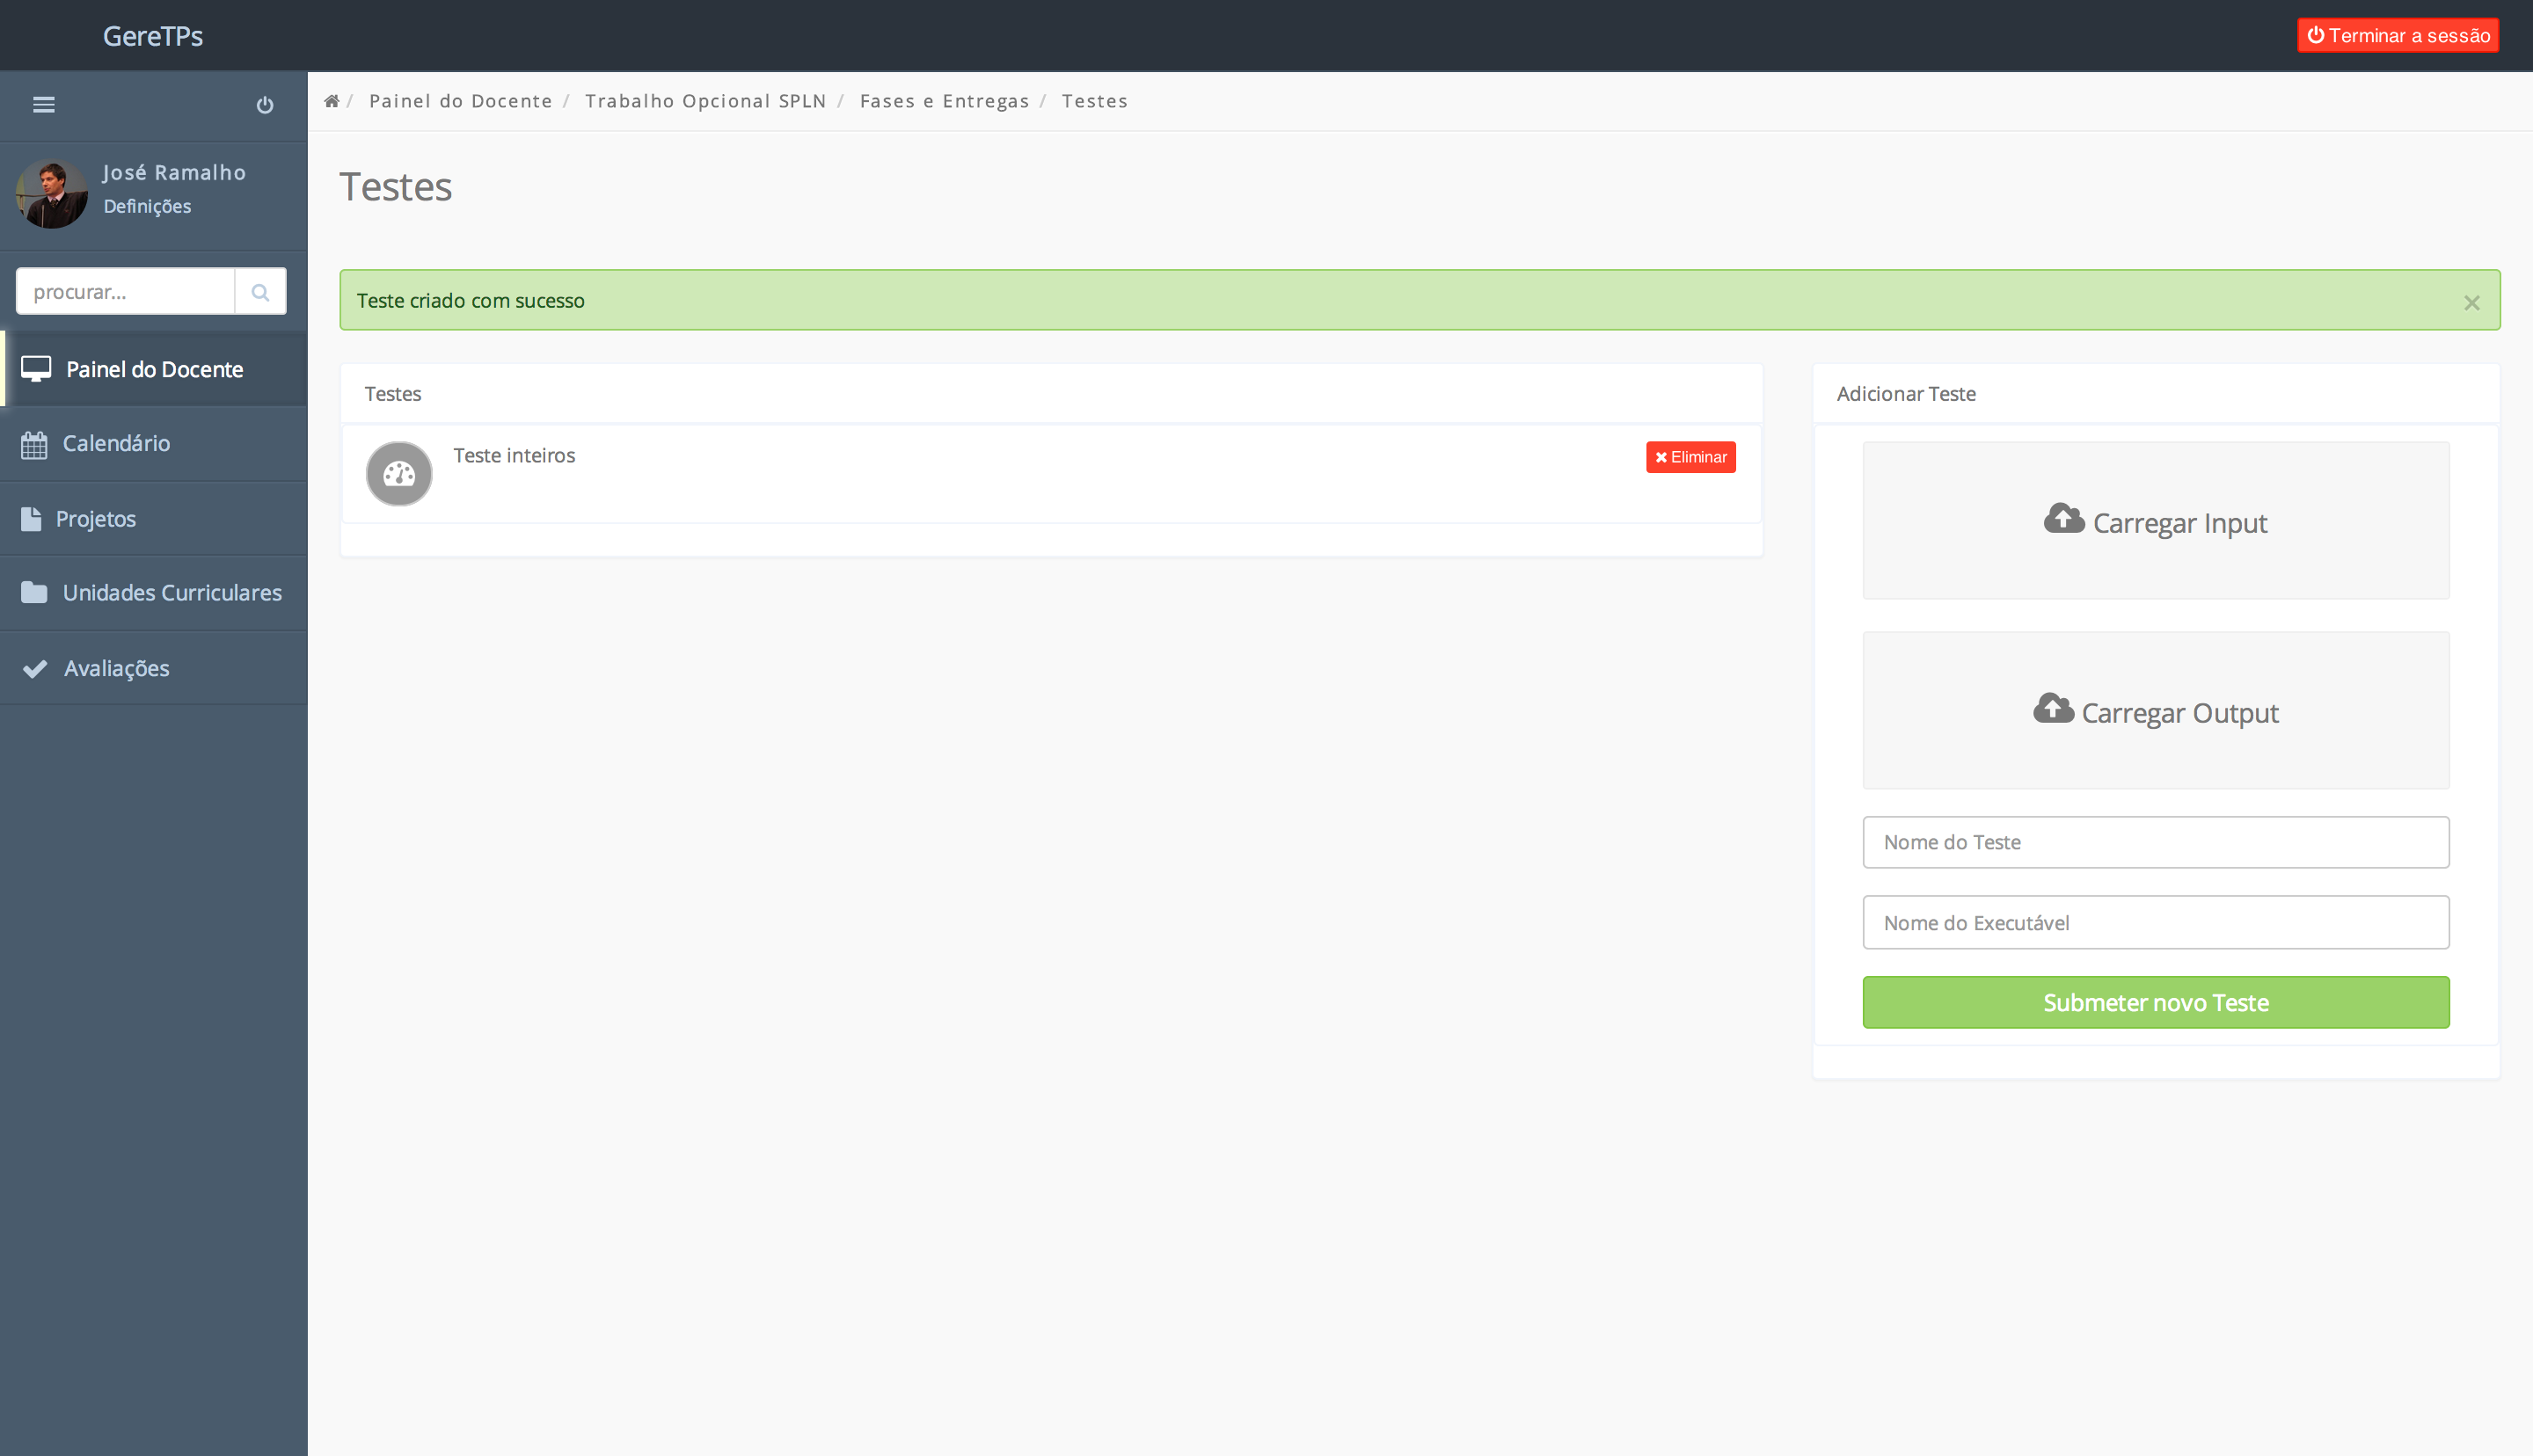
\includegraphics[width=.8\textwidth,center]{images/implementacao/docentes/testes}
  \caption{Página de criação de testes}
  \label{fig:tests}
\end{figure}

% subsubsection testes (end)
